\section{Forecast evaluation}\label{app:forecast}

Table~\ref{tab:forecast} and Fig.~\ref{fig:forecast}a summarise forecast accuracy in 2024. Averaged over horizons and sites, the direct GBM forecaster has a mean absolute error (MAE) of 31.2~gCO$_2$/kWh, against 34.4 for persistence and 40.4 for the seasonal-naive forecast. The advantage is largest at short and medium horizons: MAE falls by 23\% at 1 hour (6.2 against 8.0) and by 23\% at 6 hours (23.3 against 30.2). Beyond about 18 hours, all methods converge to the seasonal-naive level, and at 24 hours the GBM is slightly worse than the seasonal-naive benchmark. Without weather forecasts, day-ahead changes in wind output are hard to predict from the intensity history alone~\cite{maji2022carboncast}. By site, the GBM is most accurate for the volatile southern sites. In South Scotland, where intensity is low and often flat, persistence is marginally better. Diebold--Mariano tests~\cite{diebold1995comparing} with absolute-error loss and HAC variance confirm these patterns. For the three English sites, the GBM is significantly more accurate than persistence at horizons of 1--18 hours ($p\le0.001$) and indistinguishable at 24 hours ($p\ge0.13$). For South Scotland it is significantly better at 1 hour, indistinguishable at 3 hours and significantly worse from 6 hours onwards.

\begin{table}[t]
\centering
\caption{Forecast accuracy on the 2024 test year (MAE in gCO$_2$/kWh; mean over sites unless stated).}
\label{tab:forecast}
\small
\begin{tabular}{lrrrrrrr}
\toprule
 & \multicolumn{5}{c}{Horizon $h$ (hours)} & \multicolumn{2}{c}{All horizons} \\
\cmidrule(lr){2-6}\cmidrule(lr){7-8}
Model & 1 & 3 & 6 & 12 & 24 & MAE & RMSE \\
\midrule
Persistence & 8.0 & 19.3 & 30.2 & 37.4 & 40.4 & 34.4 & 48.4 \\
Seasonal naive (24 h) & 40.4 & 40.4 & 40.4 & 40.4 & 40.4 & 40.4 & 57.0 \\
Direct GBM (this study) & \textbf{6.2} & \textbf{14.9} & \textbf{23.3} & \textbf{33.9} & 42.4 & \textbf{31.2} & \textbf{41.0} \\
\bottomrule
\end{tabular}

\smallskip
\parbox{0.92\textwidth}{\footnotesize MAE by site over all horizons (persistence / GBM): South Scotland 14.1 / 16.2; North West England 24.7 / 21.8; West Midlands 56.1 / 49.3; London 42.7 / 37.6.}
\end{table}

\begin{figure}[t]
\centering
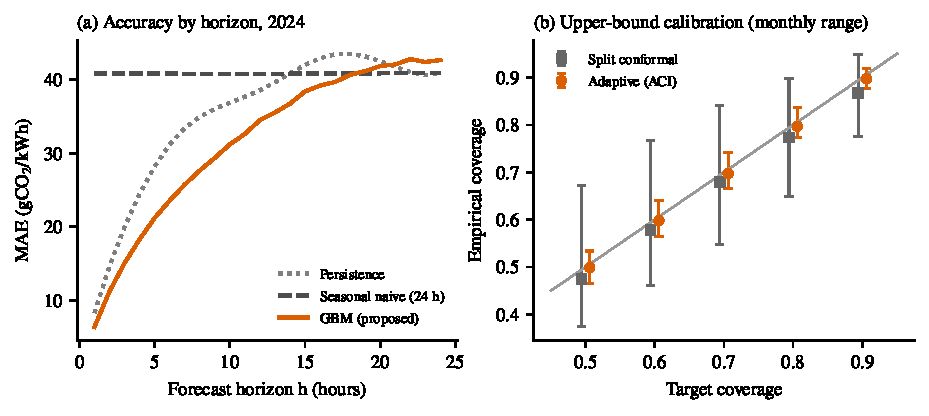
\includegraphics[width=\textwidth]{../figures/fig3_forecast.pdf}
\caption{Forecast evaluation in 2024. (a) MAE by horizon, averaged over sites. (b) Empirical coverage of one-sided upper bounds $U^\beta$ against the target level $\beta$ for static split conformal calibration and adaptive conformal inference (ACI). Markers show the annual coverage and bars the range across the 12 months.}
\label{fig:forecast}
\end{figure}

Calibration matters more than point accuracy for the risk-adjusted cost view, and Fig.~\ref{fig:forecast}b shows the effect of distribution shift. Static split-conformal bounds, calibrated on July--September 2023, under-cover in 2024 at every level: at $\beta=0.9$, annual coverage was 0.858 and monthly coverage ranged from 0.68 to 0.95. With ACI, annual coverage matches the target to within 0.002 at all levels (0.500, 0.599, 0.698, 0.798 and 0.898). Monthly coverage stays within $\pm 4$ percentage points of the target, and coverage is uniform across horizons. At $\beta=0.5$, the ACI-adjusted median lies on average 9.9~gCO$_2$/kWh below the point forecast, which reflects the downward drift in intensity that the static model does not capture. Coverage is not the whole story. In pinball loss, ACI improves on static calibration at levels 0.5--0.7 (for example 14.83 against 14.90 at 0.5) but is worse at 0.8 and 0.9 (9.06 against 8.35 at 0.9). The online recalibration buys coverage at high levels with wider bounds. Two implementation details qualify the ACI results. Feedback is delayed: the miscoverage level for horizon $h$ is updated only when the outcome is observed, $h$ hours after issue, so the adaptation lags by up to a day at long horizons. The adapted level is also clipped to $[0,1]$ and read from a quantile grid of step 0.001, so the finite-sample guarantee of ACI~\cite{gibbs2021adaptive} holds only approximately.

